\chapter{Metodologia}

A metodologia utilizada para o desenvolvimento deste trabalho buscou ter etapas de testes e validação da solução, assim buscando os melhores resultados para avaliar a sua viabilidade. Na Figura \ref{fig:metodologia} é apresentado um fluxograma ilustrando todas as etapas da metodologia abordada, além dos pontos de tomada de decisão. 

\begin{figure}[H]
    \centering
    \caption{Fluxograma das etapas executadas na metodologia}
    % 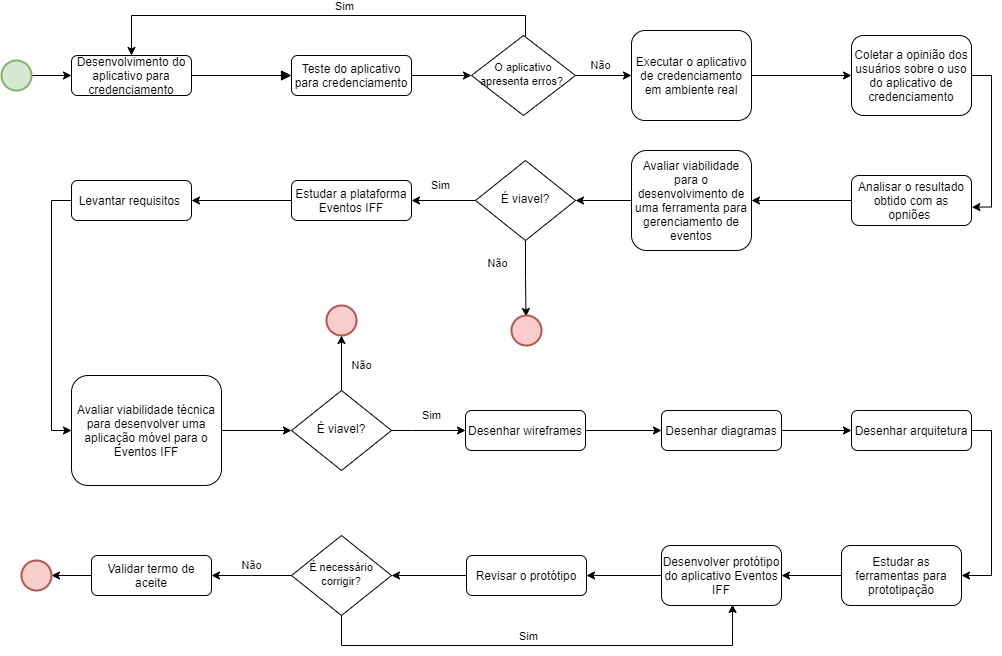
\includegraphics[scale=0.45]{figuras/metodologia.jpg}
    \fbox{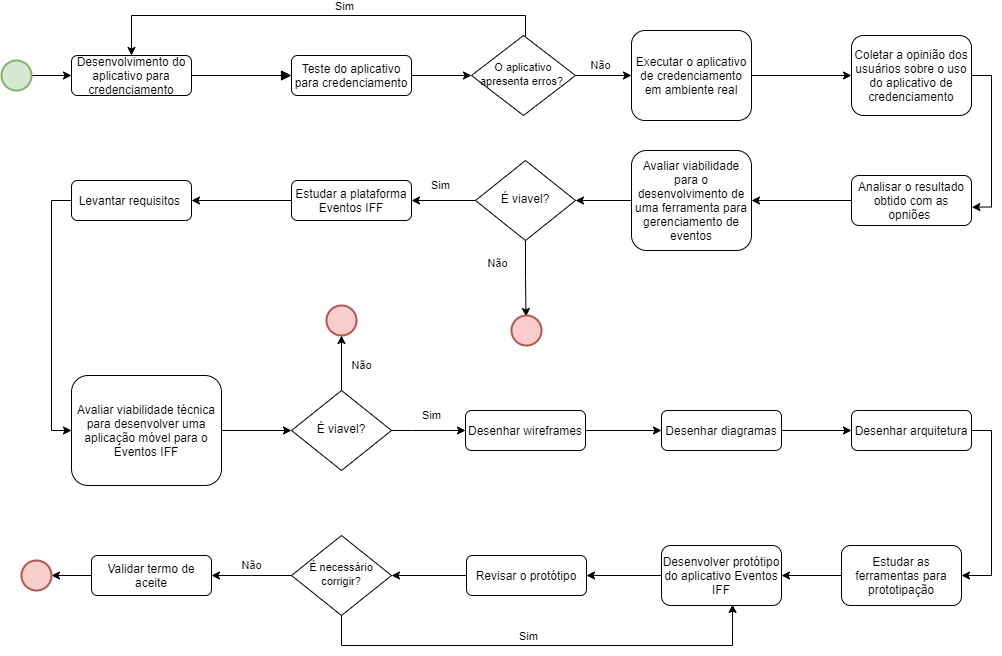
\includegraphics[scale=0.43]{figuras/metodologia.jpg}}
    \label{fig:metodologia}
    \legend{Fonte: elaborado pelos autores}
\end{figure}

Na Figura \ref{fig:metodologia}, a primeira etapa da metodologia foi desenvolver um aplicativo com a funcionalidade de credenciamento em evento. O objetivo foi validar essa funcionalidade em ambiente real. A etapa de desenvolvimento dessa ferramenta foi repetida até passar nos testes iniciais, sendo assim apta para ser utilizada no ambiente real.

Após esta etapa, foi feita uma coleta e pesquisa de opinião sobre a utilização deste aplicativo de credenciamento, e posteriormente foi feita uma análise e estudo dos resultados obtidos nesta pesquisa. Diante disso, foi possível determinar a viabilidade de desenvolver uma ferramenta para gerenciamento de eventos.

Tendo em vista a plataforma \textit{web} Eventos IFF para gerenciamento de eventos, foi feito um estudo sobre a plataforma visando ter conhecimento de suas funcionalidades e estrutura. Com isso, foi possível fazer o levantamento de requisitos com responsáveis pela plataforma e avaliar a viabilidade de desenvolver uma aplicação móvel integrada ao Eventos IFF.

Por conseguinte, foi iniciada a etapa de desenho da solução, fazendo o desenho dos \textit{wireframes}, diagramas e arquitetura. Essa etapa teve como objetivo ter um esclarecimento das funcionalidades que a solução possuiria, além de como se comunicaria com o Eventos IFF.

Decorrente do desenho da solução e mapeamento das funcionalidades feitas na etapa anterior, foi iniciado o estudo das ferramentas no mercado próprias para construção de protótipos interativos. Após a escolha da ferramenta, foi iniciado o desenvolvimento do protótipo da solução. Essa etapa de desenvolvimento foi repetida até que o protótipo estivesse adequado a solução desenhada e proposta. Dessa forma, finalizando as etapas dessa metodologia, foi feita a validação do termo de aceite.
